\documentclass[10pt,twocolumn,letterpaper]{article}

\usepackage{cvpr}
\usepackage{times}
\usepackage{epsfig}
\usepackage{graphicx}
\usepackage{amsmath}
\usepackage{amssymb} 
\usepackage{multirow}
\usepackage{hhline}
\usepackage{subfigure}

% Include other packages here, before hyperref.

% If you comment hyperref and then uncomment it, you should delete
% egpaper.aux before re-running latex.  (Or just hit 'q' on the first latex
% run, let it finish, and you should be clear).
\usepackage[pagebackref=true,breaklinks=true,letterpaper=true,colorlinks,bookmarks=false]{hyperref}

 \cvprfinalcopy % *** Uncomment this line for the final submission

\def\cvprPaperID{} % *** Enter the CVPR Paper ID here
\def\httilde{\mbox{\tt\raisebox{-.5ex}{\symbol{126}}}}

% Pages are numbered in submission mode, and unnumbered in camera-ready
\ifcvprfinal\pagestyle{empty}\fi

\begin{document}

%%%%%%%%% TITLE
%%\title{A Novel Computer Aided Method \\ 
%%           to Classify Lung Nodules in Thoracic CT Scans}

\title{Review of:\\
The All Convolutional Net}


\author{
SiKai Lee\\
Columbia University\\
116th St \& Broadway, New York, NY, USA\\
{\tt\small sikai.lee@columbia.edu}
\and
ZhiHao Luo\\
Columbia University\\
116th St \& Broadway, New York, NY, USA\\
{\tt\small zl2463@columbia.edu}
\and
Juan Pablo Colomer\\
Columbia University\\
116th St \& Broadway, New York, NY, USA\\
{\tt\small jpc2192@columbia.edu}
}
\maketitle

\begin{abstract} 
We review Striving for Simplicity: The All Convolutional Net by Jost Tobias Springenberg, Alexey Dosovitskiy, Thomas Brox, and Martin Riedmiller. Conventionally, convolutional neural nets (CNN) are built by alternating convolutional and max-pooling layers together with a few fully connected layers and a softmax layer at the end. However, state-of-the-art convolutional architectures have increasingly deviated the above model which begs the question of which components of a conventional convolutional net are responsible for achieving state-of-the-art performance. The authors demonstrate that the pooling function can be represented with the convolutional function and show that nets made out of only convolutional layers and a softmax layers can produce results comparable to, if not better than state-of-the-art performance on several object recognition datasets. They also introduce a new variant of the 'deconvolution approach' for visualizing features learned by CNNs that are applicable to a broader range of network structures. 

Here, we replicate the neural nets proposed in the paper and attempt to visualize the first three layers of the neural net consisting of only convolutional layers and a softmax layer with the guided backpropagation method.
\end{abstract} 
\section{Review}
\subsection{Convolutional Neural Nets Background}
In recent years, Convolutional Neural Nets (CNNs) have become more and more popular for image related tasks. First introduced by Yann Lecun, this particularly powerful neural network structure has become wide adopted by researches for their efficiency and robustness. Over the years, multiple papers attempts to improve performance of the CNN by changing activation functions or by augmenting the structure. However, most designs seem to share the same principle: they use alternating convolution and max-pooling layers followed by some number of fully connected layers. A typical convolution maxpooling sequence is shown in figure \ref{fig:cnn}. \\
\begin{figure}[hb]
	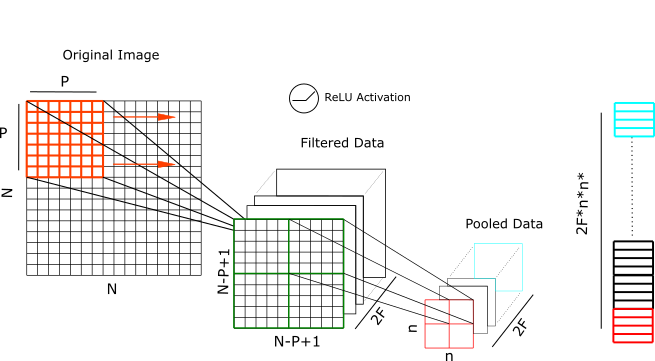
\includegraphics[width = 8cm]{img/CNN.png}
    \caption{\label{fig:cnn}
    An example architecture of a CNN.
    On the left is an 2D image input, followed by a convolutional layers, and a 
    max pooling layer. }
\end{figure}\\
The convolution layers defines a set of filters and an activation function. It convolve the input to that layer with its filters to generate an output which is then passed through the activation function. In this example, the convolution layer contains $2F$ filters of size $P\times P$; by convolving the $N\times N$ input with all of its filters, it generate $2F$ feature maps with size $(N-P+1)\times (N-P+1)$. The final output of the convolution layers are obtained by passing the feature maps through the ReLU function.
\begin{align}
	ReLU(x) = max(0,x)
\end{align}
The max-pooling layer down-scales the feature maps by dividing the feature maps into subsections and representing that entire subsection with the maximum value inside it.\\
Finally, at the end of the last max-pool layer, the feature maps are flattened into a vector which are usually used as the input to the fully connected layers are shown in Figure \ref{fig:fullyconnected}\\
In the fully connected layers, each node has a weighted connection to every node from the previous layer, it's output is determined by passing through the weighted sum of previous layer output through an activation function. The input is non-linear transformed through the layers and this non-linear transformation helps the neural net in finding separation between classes.\\
\begin{figure}[hb]
	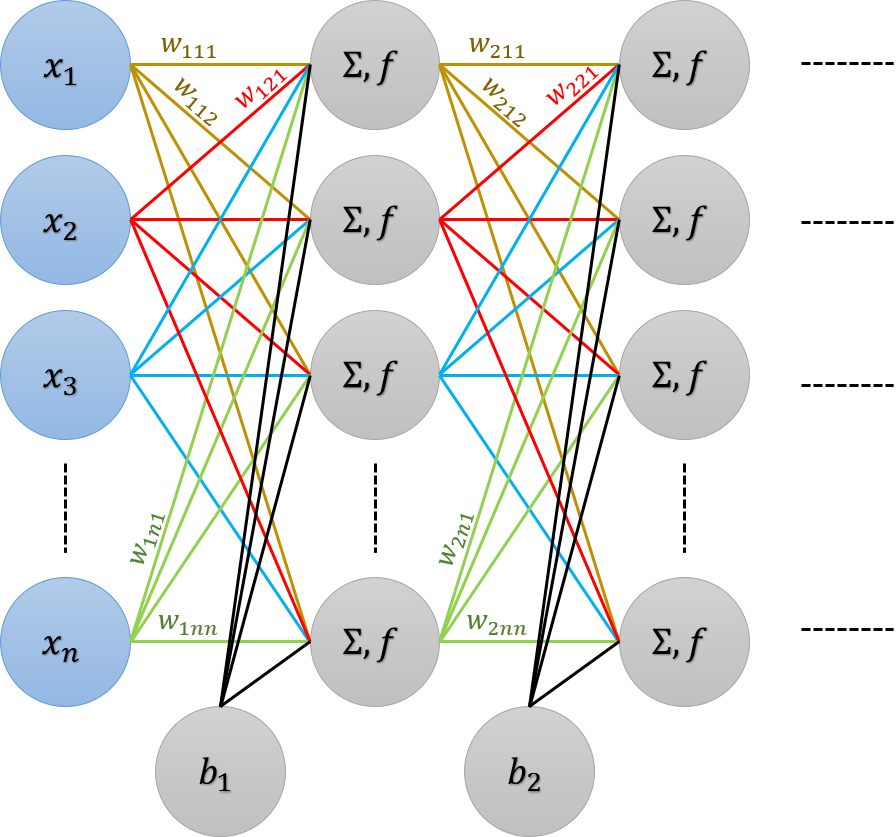
\includegraphics[width = 8cm]{img/fullyconnected.png}
    \caption{\label{fig:fullyconnected}
    Fully connected layers}
\end{figure}

\subsection{Homogeneous Structure}
The author challenges the conventional CNN structure by introducing a number of models that are increasing more homogeneous -- the most extreme of which contains only convolutional layers without pooling or fully connected layers.
According to the paper a pooling layer is equivalent to perform a feature-wise convolution by replacing the activation function with a $p$-norm. Thus, they question why a pooling layer is needed. Based on this questioning
they state the hypothesis that pooling is only important in order to reduce the dimensionality. Assuming this hypothesis is true, a pooling layer can be replaced by
a convolutional layer with an increased stride.

Additionally, by using convolutional layers with a filter size smaller than 5, the authors reduce the number of parameters in a network.
Moreover, they argument that fully connected layers are not necessary since units in the last convolutional layer in the network cover a sufficient portion of the image to be able to recognize it.
% Please proofread what I've written above

\section{Experiments}

\subsection{Architectures}
% Check these architectures
\begin{table}
  \centering
  \begin{tabular}{|c|c|c|c|}
    \hline
    Model A & Strided-CNN-A & ConvPool-CNN-A & ALL-CNN-A \\
    \hline
    \multicolumn{4}{|c|}{Input $32\times32$ RGB Images} \\
    \hline
    $5\times5$ conv. 96 ReLU & $5\times5$ conv. 96 ReLU stride 2 &  $5\times5$ conv. 96 ReLU & $5\times5$ conv. 96 ReLU \\
    & & $3\times3$ conv. 96 ReLU & \\
    \hline
    $3\times3$ max-pooling stride 2 & & $3\times3$ max-pooling stride 2& $3\times3$ conv. 96 ReLU stride 2 \\
    \hline
    $5\times5$ conv. 192 ReLU & $5\times5$ conv. 192 ReLU stride 2 &  $5\times5$ conv. 192 ReLU & $5\times5$ conv. 192 ReLU \\
    & & $3\times3$ conv. 192 ReLU & \\
    \hline
    $3\times3$ max-pooling stride 2 & & $3\times3$ max-pooling stride 2& $3\times3$ conv. 96 ReLU stride 2 \\
    \hline
    \multicolumn{4}{|c|}{$3\times3$ conv. 192 ReLU} \\
    \multicolumn{4}{|c|}{$1\times1$ conv. 192 ReLU} \\
    \multicolumn{4}{|c|}{$1\times1$ conv. 10 ReLU} \\
    \multicolumn{4}{|c|}{global average pooling layer} \\
    \multicolumn{4}{|c|}{10-way softmax} \\
  \end{tabular}
  \caption{Architectures for Model A}
\end{table}

\begin{table}
  \centering
  \begin{tabular}{|c|c|c|c|}
    \hline
    Model B & Strided-CNN-B & ConvPool-CNN-B & ALL-CNN-B \\
    \hline
    \multicolumn{4}{|c|}{Input $32\times32$ RGB Images} \\
    \hline
    $5\times5$ conv. 96 ReLU & $5\times5$ conv. 96 ReLU &  $5\times5$ conv. 96 ReLU & $5\times5$ conv. 96 ReLU \\
    $1\times1$ conv. 96 ReLU & $1\times1$ conv. 96 ReLU stride 2 &  $1\times1$ conv. 96 ReLU & $1\times1$ conv. 96 ReLU \\
    & & $3\times3$ conv. 96 ReLU & \\
    \hline
    $3\times3$ max-pooling stride 2 & & $3\times3$ max-pooling stride 2& $3\times3$ conv. 96 ReLU stride 2 \\
    \hline
    $5\times5$ conv. 192 ReLU & $5\times5$ conv. 192 ReLU &  $5\times5$ conv. 192 ReLU & $5\times5$ conv. 192 ReLU \\
    $1\times1$ conv. 192 ReLU & $1\times1$ conv. 192 ReLU stride 2 &  $1\times1$ conv. 192 ReLU & $1\times1$ conv. 192 ReLU \\
    & & $3\times3$ conv. 192 ReLU & \\
    \hline
    $3\times3$ max-pooling stride 2 & & $3\times3$ max-pooling stride 2& $3\times3$ conv. 96 ReLU stride 2 \\
    \hline
    \multicolumn{4}{|c|}{$3\times3$ conv. 192 ReLU} \\
    \multicolumn{4}{|c|}{$1\times1$ conv. 192 ReLU} \\
    \multicolumn{4}{|c|}{$1\times1$ conv. 10 ReLU} \\
    \multicolumn{4}{|c|}{global average pooling layer} \\
    \multicolumn{4}{|c|}{10-way softmax} \\
  \end{tabular}
  \caption{Architectures for Model B}
\end{table}

\begin{table}
  \centering
  \begin{tabular}{|c|c|c|c|}
    \hline
    Model C & Strided-CNN-C & ConvPool-CNN-C & ALL-CNN-C \\
    \hline
    \multicolumn{4}{|c|}{Input $32\times32$ RGB Images} \\
    \hline
    $3\times3$ conv. 96 ReLU & $3\times3$ conv. 96 ReLU &  $3\times3$ conv. 96 ReLU & $3\times3$ conv. 96 ReLU \\
    $3\times3$ conv. 96 ReLU & $3\times3$ conv. 96 ReLU stride 2 &  $3\times3$ conv. 96 ReLU & $3\times3$ conv. 96 ReLU \\
    & & $3\times3$ conv. 96 ReLU & \\
    \hline
    $3\times3$ max-pooling stride 2 & & $3\times3$ max-pooling stride 2& $3\times3$ conv. 96 ReLU stride 2 \\
    \hline
    $3\times3$ conv. 192 ReLU & $3\times3$ conv. 192 ReLU &  $3\times3$ conv. 192 ReLU & $3\times3$ conv. 192 ReLU \\
    $3\times3$ conv. 192 ReLU & $3\times3$ conv. 192 ReLU stride 2 &  $3\times3$ conv. 192 ReLU & $3\times3$ conv. 192 ReLU \\
    & & $3\times3$ conv. 192 ReLU & \\
    \hline
    $3\times3$ max-pooling stride 2 & & $3\times3$ max-pooling stride 2& $3\times3$ conv. 96 ReLU stride 2 \\
    \hline
    \multicolumn{4}{|c|}{$3\times3$ conv. 192 ReLU} \\
    \multicolumn{4}{|c|}{$1\times1$ conv. 192 ReLU} \\
    \multicolumn{4}{|c|}{$1\times1$ conv. 10 ReLU} \\
    \multicolumn{4}{|c|}{global average pooling layer} \\
    \multicolumn{4}{|c|}{10-way softmax} \\
  \end{tabular}
  \caption{Architectures for Model C}
\end{table}

\begin{table}
  \centering
  \begin{tabular}{|c c c|}
    Model & Error (\%) & # parameters \\
    \hline
    Model A & 12.47\% & \approx 0.9 M \\
    Strided-CNN-A & 13.46\% & \approx 0.9 M \\
    ConvPool-CNN-A & 10.21\% & \approx 1.28 M \\
    ALL-CNN-A & 10.30\% & \approx 1.28 M \\
    \hline
    Model B & 10.20\% & \approx 1 M \\
    Strided-CNN-B & 10.98\% & \approx 1 M \\
    ConvPool-CNN-B & 9.33\% & \approx 1.35 M \\
    ALL-CNN-B & 9.10\% & \approx 1.35 M \\
    \hline
    Model C & 9.74\% & \approx 1.3 M \\
    Strided-CNN-C & 10.19\% & \approx 1.3 M \\
    ConvPool-CNN-C & 9.31\% & \approx 1.4 M \\
    ALL-CNN-C & 9.08\% & \approx 1.4 M \\
  \end{tabular}
  \caption{Original classification Error on CIFAR-10}
\end{table}

\section{Discussion}
\begin{table}[H]
  \centering
  \begin{tabular}{|c c c c|}
    \hline
    Model & Error (\%) &  Run Time & Learn Rate\\
    \hline
    Model A & 15.16\% &   343.63m & 0.05\\
    Strided-CNN-A & 18.23\% &  168.89m  & 0.05\\
    ConvPool-CNN-A & 11.44\% &  694.26m & 0.05 \\
    ALL-CNN-A & 12.47\% &  642.76m  & 0.01\\
    \hline
    Model B & 13.52\% & 453.42  & 0.05\\
    Strided-CNN-B & 15.56\% & 440.26 & 0.05 \\
    ConvPool-CNN-B & 11.84\% & 879.25 & 0.01 \\
    ALL-CNN-B & 11.84\% & 626.85 &  0.01 \\
    \hline
    Model C & 11.11\% &    708.42m & 0.05 \\
    Strided-CNN-C & 12.91\% &   428.63m & 0.05 \\
    ConvPool-CNN-C & 11.09\% &   1346.35m & 0.01 \\
    ALL-CNN-C &  11.17\% &   984.55m & 0.05 \\
    \hline
  \end{tabular}
  \caption{Reproduced errors on CIFAR-10}
  \label{tab:ourResults}
\end{table}
After running experiments on the 12 models listed in Tables \ref{tab:modelA}, \ref{tab:modelB}, and \ref{tab:modelC}, we obtain the above results in Table \ref{tab:ourResults}.

In this section, we discuss the most important factors that contributed to us achieving close to state-of-the-art performance such as data preprocessing and learning rate decay. We also explain how and why there was a performance gap between our results and those detailed in the paper.

\subsection{Data Preprocessing}
The importance of data preprocessing cannot be overstated. Using an unpreprocessed dataset usually result in untrainable neural net. Here, we elaborate on a few of the most important preprocessing procedure we learned from this project.
\subsubsection{Input Value Normalization}
    The CIFAR-10 dataset contains 32x32x3 RGB images flattened into vectors of 3072. Like typical RGB images, the values encoded in uint8 which are integers ranging from 0 to 255. However, having large values were detrimental to the training process. Since the input is included in the calculating back-propagation, large values quickly cause the gradient decent to "overstep" by taking steps that are too large at each iteration. In our case, it caused the variable holding the network loss to overflow, resulting in "NaN" losses which completely halts the training process.
    
\subsubsection{Centering}
    Centering of the input data is the next crucial step in preprocessing. In fact, if we only normalized the input values without centering, the learning process would not get anywhere. In the case of the above experiments, it resulted in a uniform probability vector across the 10 target classes irregardless of which of the 12 models/architectures used. This suggested that the classifier networks were continuously driven towards the same local minimum where every class is equally likely. In other words, none of the 12 classifiers was able to extract any meaningful information from the input, and they were not able to learn a separating plane between the classes in the input space.
    
    An intuitive explanation as to why this happens is that: a 2-D cluster of points which may otherwise be linearly separated when centered at the origin may create more complexity when the points are biased in some direction. Hence two additional bias terms are needed to find the new separating plane. With an input with dimension 3072 with multiple convolutional layers and only 1 bias term per layer, it is clear that if the input data does not have mean of 0, the network would have trouble finding separation between classes.
    
    A more technical explanation is if all the input values are in the positive region, the weights will try to push the values down in order to perform meaningful learning. However, as soon as the output values becomes negative, the ReLU activation would force the values to zero. Eventually, the gradient would drive all intermediate-layer output value to zero which we confirmed. These zero values gets propagated to the very last layer right before softmax. With ten 0 values, the softmax returns a vector of length 10, where each value is 0.1 denoting the probability of the output classes. Since the intermediate values are zeros, the network stops learning and the weights are no longer updated.
    
    After applying centering by subtracting the overall mean from the training data, learning progresses. However, the error rate (for model A) only drops to 43\% (compared to the 15.16\% we obtained eventually).
    
\subsubsection{Whitening and Contrast Normalization}
    Whitening is the process that reduces correlation between different inputs. So a whitened image would have a covariance matrix that is very close to the identity matrix. Intuitively, we can think of whitening as reducing redundant information in the input, which allow the CNN to learn more or less "independent" features, that are more helpful in classification. In fact, a whitening-like process takes place in the human eye as well in an attempt to convey only useful information and reducing redundancy. Even though the whitened image does not look particularly recognizable to the human eyes, it helps the CNN to achieve a much better accuracy when used for training.
    
    Global contrast normalization is another important procedure that we performed. This is done by dividing the standard deviation from the dataset \cite{coates2011analysis}. This effectively transform all the inputs to be in the same input space, and allows for effective learning.\\
    For reference, we have included an image from the CIFAR-10 dataset and its whitened-and-contrast-normalized counterpart.
    \begin{figure}[hb]
    	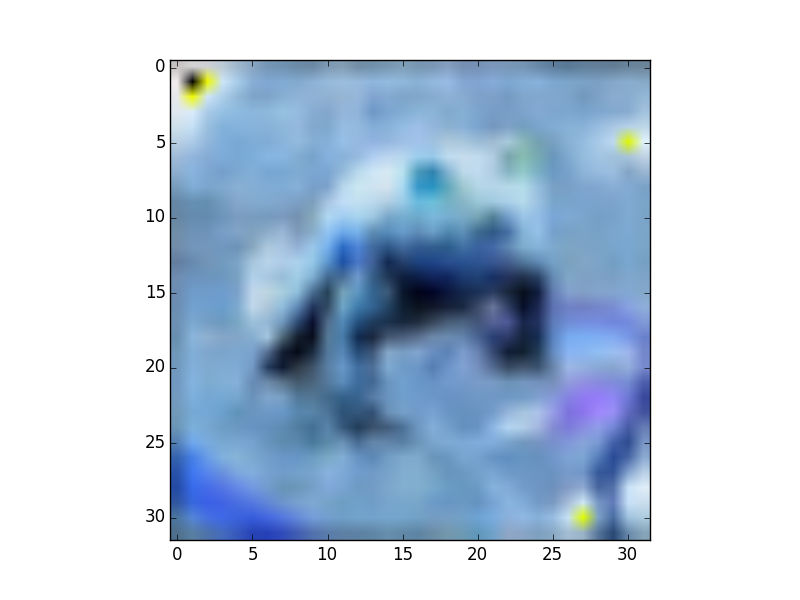
\includegraphics[width = 4cm]{img/frog.png}
    	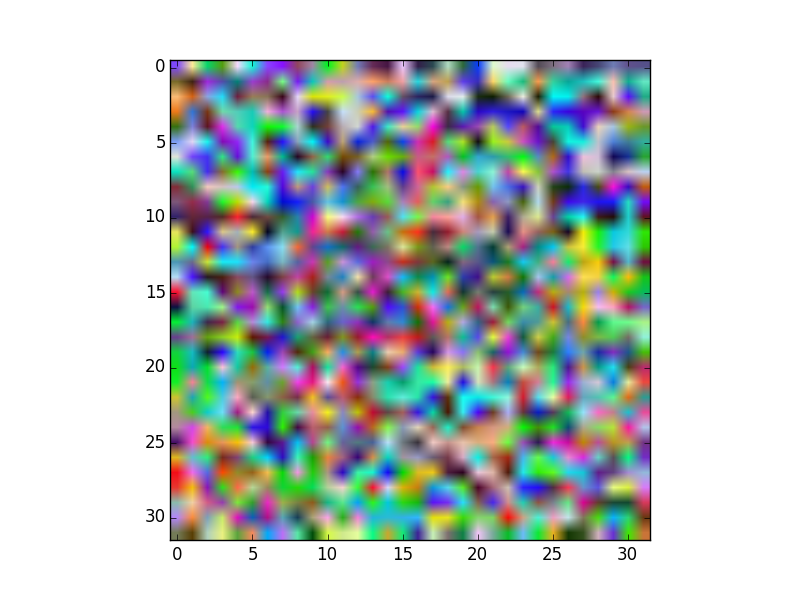
\includegraphics[width=4cm]{img/frog_whitened.png}
    	\caption{An image of a frog before whitening and contrast normalization (left) and after (right)}
    	\label{fig:frog}
    \end{figure}\\

\subsection{Learning Rate}
    Learning rate has always been an important hyper-parameter in training. In this project, we found that having a high learning rate (especially in the beginning) is detrimental to the learning process; in particular, similar to the value-normalization problem, a high learning rate cause the update to "over-step" and eventually cause the loss to overflow so it actually led the learning process away fro objective.
    \subsubsection{Rate Decay}
        We also note the importance of having a decaying learning rate. In this experiment, learning happens very quickly in the beginning. For most of the 12 models, learning comes to a bottleneck after 100 epochs. By letting the learning rate to shrink to 10\% of its original value at the bottleneck, the error rate continues to drop. As mentioned in section on implementation, we implemented learning rate decay at 3 checkpoints as the paper suggested.
        
        
\subsection{Filter Map Visualization} 
    In this section we present the visualization of the filter map of 2 selected convolutional layers. The layers are chosen to be the top 2 layers from the All CNN C model. We are using the top layers since the filters there has more intuitive explanations.
     \begin{figure}[hb]
    	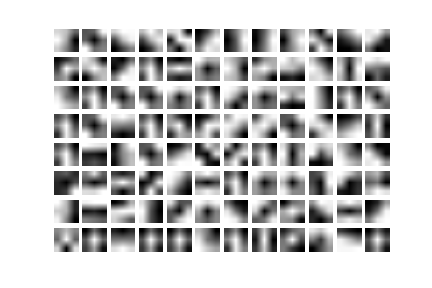
\includegraphics[width = 8cm]{img/conv1_1.png}
    	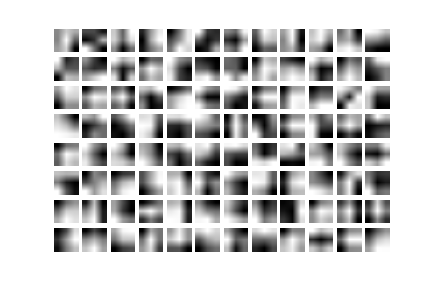
\includegraphics[width=8cm]{img/conv1_2.png}
    	\caption{Visualization of the first (top) and 2nd layer (bottom) filters of the All Convolution C model}
    	\label{fig:frog}
    \end{figure}
    
    Each layer has 96 filters, we are only looking at the first dimension of the filters. From the figure it is reasonably clear that many of the filters are edge detectors and that they are separated by 45 degree angles. This provies good separation while ensuring that the image edge with different angles are detected.
\subsection{Performance Gap}
In this subsection, we address the reasons for the performance gap between our results and the ones achieved by the paper.

There are several implementation details and hyper-parameters that the paper did not detail: batch size, optimal learning rate, layer padding, and the global averaging layer implementation. While some of these had a lesser effect on final performance, a number of these had significant effect on the training process.

\subsubsection{Batch Size}
The batch size used during stochastic gradient descent determines the "randomness" of the gradient at every iteration. Having a larger batch size means that there is less randomness in the gradient since it is an average of more numbers of training samples; on the other hand, if the gradient is computed using a small number of training samples, the gradient is likely to be biased, so the learning process would be highly dependent on training sample batch size.

While the gradient computed using a large number of training data is more stable and closer to the true gradient, a more random gradient, along with the use of momentum, enables the network to get out of local minimas (since the combined gradient might lead the training in different directions).

However, this crucial hyper-parameter choice is missing from the paper so we used a batch size of 200 from small-scale experiments and past experience.

\subsubsection{Learning Rate}
The optimal learning rate for each model was not presented. Instead, the paper offered 4 candidate learning rates. Given that each experiment ran on average for at least 10 hours, we tried the smallest value 0.01 for each model and the second smallest value of 0.05. When there was no noticeable improvement in the cost function, we stopped experimenting with larger learning rates due to time constraints since trying another learning rate would mean at least 12 more experiments. However, there is no guarantee that an even larger learning rate (0.1 or 0.25) will not improve performance. Hence, this is an important factor in accounting for the performance gap between our results and the papers.

\subsection{Convolution Details}
There are several details in the convolution layer that are missing: padding and ignore-border parameters.
\subsubsection{Padding}
Normally if there are a large number of convolutional layers, the images at each layer is padded to avoid diminishing the image dimension too quickly. In fact, in model B, if there was no padding, each feature map input to the last layer would have a dimension of only $2\times 2$. However, whether the authors added padding to the layers and to which layers, are not known. We added padding to most layers as mentioned previously in the implementation section.

\subsubsection{Ignore Border}
The ignore border parameter is also missing from the paper. A change in this parameter could cause the filter to ignore the last few values in an image dimension which could possibly cause a small loss of border information.

\subsection{Global Averaging Layer}
Typically in a global averaging layer, each feature map is reduced to its average. So a global averaging layer taking an input of feature maps with dimensions of $M\times N \times 10$ (where $N$ and $M$ can be anything) would have an output of dimension $1\times 1\times 10$. However, it is confusing that the authors associated the global averaging layer has a dimension of $6\times6$ since the layer does not have internal filters. In our implementation, we simply ignored that and implemented a normal global averaging layer.




{\small
\bibliographystyle{ieee}
\bibliography{Bib}
}


\end{document}
